\documentclass[11pt]{scrartcl}

\RequirePackage{tikz}
\RequirePackage{pgf-pie}
\usepackage{subcaption}

\begin{document}

\fbox{
    \begin{minipage}{\linewidth}
        \centering
            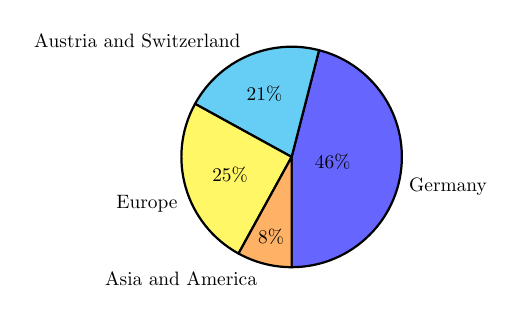
\begin{tikzpicture}[scale=.7, every node/.style={scale=0.7}] % Tikz environment
                \pie[rotate=270, radius=2]
                {46/Germany, 21/Austria and Switzerland, 25/Europe, 8/Asia and America}
            \end{tikzpicture}
        \captionof{figure}{Revenue by Geographic}
    \end{minipage}
}

\begin{minipage}{.45\linewidth}
    \centering
        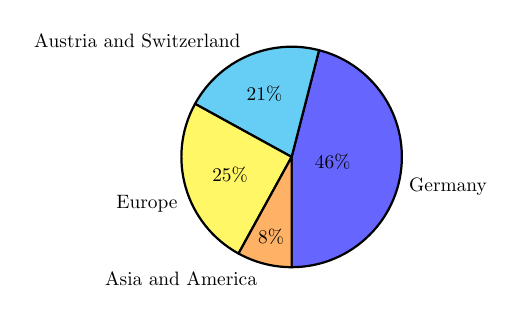
\begin{tikzpicture}[scale=.7, every node/.style={scale=0.7}] % Tikz environment
            \pie[rotate=270, radius=2]
            {46/Germany, 21/Austria and Switzerland, 25/Europe, 8/Asia and America}
        \end{tikzpicture}
    \captionof{figure}{Revenue by Geographic}
\end{minipage}

\begin{figure}[h!]
    \fbox{\begin{subfigure}[b]{.45\linewidth}
        \centering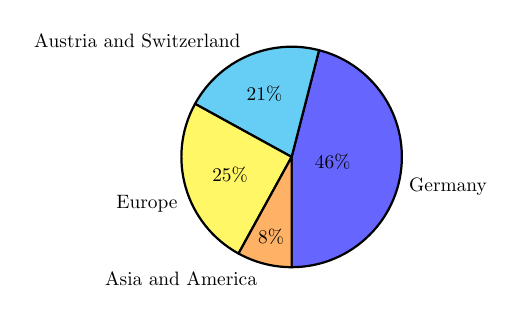
\begin{tikzpicture}[scale=.7, every node/.style={scale=0.7}] % Tikz environment
        \pie[rotate=270, radius=2]
        {46/Germany, 21/Austria and Switzerland, 25/Europe, 8/Asia and America}
        \end{tikzpicture}
        \caption{A subfigure}\label{fig:1a}
    \end{subfigure}}%
    \hfill
    \fbox{\begin{subfigure}[b]{.45\linewidth}
        \centering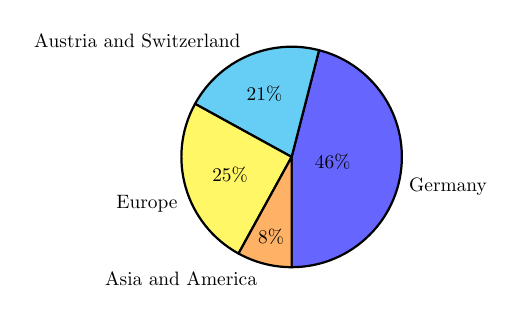
\begin{tikzpicture}[scale=.7, every node/.style={scale=0.7}] % Tikz environment
        \pie[rotate=270, radius=2]
        {46/Germany, 21/Austria and Switzerland, 25/Europe, 8/Asia and America}
        \end{tikzpicture}
        \caption{Another subfigure}\label{fig:1b}
    \end{subfigure}}
    \caption{A figure}\label{fig:1}
\end{figure}

\end{document}